% !TEX program = xelatex
\documentclass[a4paper,12pt]{article}

% Essential packages
\usepackage{geometry}
\usepackage{graphicx}
\usepackage{xeCJK}
\usepackage{titlesec}
\usepackage{booktabs}
\usepackage{listings}
\usepackage{float}
\usepackage{hyperref}
\usepackage{enumitem}
\usepackage{fancyhdr}
\usepackage{lastpage}
\usepackage{amsmath}

% Page geometry
\geometry{
    top=25mm,
    bottom=25mm,
    left=25mm,
    right=25mm
}

% Header and footer style
\pagestyle{fancy}
\fancyhf{}
\fancyhead[R]{\thepage\ of \pageref{LastPage}}
\renewcommand{\headrulewidth}{0pt}

% Title formatting
\titleformat{\section}
  {\normalfont\Large\bfseries}{\thesection}{1em}{}
\titleformat{\subsection}
  {\normalfont\large\bfseries}{\thesubsection}{1em}{}

% Code listing style
\lstset{
    basicstyle=\small\ttfamily,
    numbers=left,
    numberstyle=\tiny,
    frame=single,
    breaklines=true
}

% Document info
\title{
    
\includegraphics[width=0.4\textwidth]{ysu-logo.png}\\[1cm] % logo
    {\LARGE Proposal For ASC 25}\\[0.5cm]
    \large Team Name: YSU Super Fighters\\[1cm] % 使用占位符
    \begin{tabular}{c}
        \large Jin Chenye \\
        \large Li Wangyang \\
        \large Cui Shuyang \\
        \large Li Jinze \\
        \large Fang Yi
    \end{tabular}
}
\author{}
\date{\vfill January 8, 2025}

\begin{document}

\maketitle
\thispagestyle{empty}
\vfill
\begin{center}
    \textit{A proposal submitted to the ASC 25 committee}
\end{center}
\newpage

\tableofcontents
\addtocontents{toc}{\protect\enlargethispage{\baselineskip}}
\newpage

\section{Brief Background Description of Supercomputing Activities}

\subsection{Hardware and Software Platforms}
Our university established a high-performance computational (HPC) cluster in 2017, named Super Center Center of Yanshan University, through the integration of supercomputer resources in the university. The center contains a total of 36 nodes, 896 available computing cores, a total of 2.176TB of memory and 33TB of available storage capacity. Its theoretical double-precision floating point performance peaks at 28.672 trillion times per second. At Yanshan University, it is the highest-performance high-performance computing cluster with the largest computing capacity, the highest computing power and the most professional operation and maintenance team. It provides super computing environmental protection for national and provincial-level scientific research projects undertaken by the research teams of other colleges. As of March 9, 2018, the total cost of the supercomputer CPU was 2963096203 seconds and 335 I jobs were scheduled. At present, after more than six months of trial operation, our school has accumulated rich experience in daily operation management, technical support, application services and personnel training of supercomputer centers.

The supercomputing center adopts a mature and general system architecture, which can be used to compute core 896 Cores, total memory of 2.112tb, and 33TB of storage capacity, which can be applicable to various types of applications. The main configurations are as follows:

\begin{table}[H]
\centering
\caption{The main configurations}
\begin{tabular}{|l|l|l|l|}
\hline
Type & Number(Desk) & Name & Description \\
\hline
Management & 1 & mgt1 &  \\
\hline
Login node & 1 & login &  \\
\hline
Compute node & 30 & node1-node30 & 2 Intel E5-2683v3 processors ( 28 Cores 2.0Ghz) \\
 &  &  & 64GB DDR4 ECC REG memory \\
 &  &  & Infiniband QDR 40Gb/s high-speed network \\
\hline
GPU Visual Node & 2 & GPU1,GPU2 & 2 Intel E5-2683v3 Processors ( 28 Cores 2.0Ghz) \\
 &  &  & 128GB DDR4 ECC REG memory \\
 &  &  & Infiniband QDR 40Gb/s high-speed network \\
 &  &  & NVIDIA TitanX GPU \\
\hline
IO node & 2 & gpfs1,nfs & Gpfs1 capacity available 18TB available 15TB,nfs capacity \\
\hline
\end{tabular}
\end{table}

The Supercomputing center supports the running of computing software such as Ansys, Fluent, Vasp, Lammps, Comsol, and supports the compiling and running environment of C(C++), Fortran and other languages to ensure the computational requirements of self-compiled applications. Software resources are listed as follows:

\begin{table}[H]
\centering
\caption{Software resources}
\begin{tabular}{|l|l|l|}
\hline
number & Software Name & Description \\
\hline
1 & Centos7.2 & Operating System Platform \\
\hline
2 & NFSv4 & Web file system \\
\hline
3 & MPICH/MPICH2/OpenMPI & Open source parallel development environment \\
\hline
4 & Paramon Paratune & Application of running feature collector Application of running feature analyzer \\
\hline
5 & Intel Parallel Studio XE 2015 & Intel Parallel Development Suite \\
\hline
6 & Intel MKL 2017 & Intel Library of Mathematical Functions \\
\hline
7 & Intel MPI 2017 & Intel Parallel Messaging Library \\
\hline
8 & IBM Platform Computing LSF & Resource Management and Operational Movement Control System \\
\hline
9 & IBM GPFS & Common Parallel Document System \\
\hline
10 & Openmpi 2.0.2 & Open source Intel Parallel Messaging Library \\
\hline
11 & FFTW & Fuliye \\
\hline
12 & gromacs-5.1.4 & Molecular dynamics program \\
\hline
\end{tabular}
\end{table}


\subsection{Supercomputing-related Courses, Trainings, and Interest Groups}
Our school has an organization of supercomputers, including parallel computing group, algorithm design and optimization group, Linux cluster construction group and test group. In the parallel computing group, the leading teachers teach relevant knowledge, and students learn parallel programming, C language, MPI, cluster management and other parallel computing knowledge independently. In addition, our school has set up a discussion group for students who like supercomputers. We learn from each other in the discussion group. Students who have experience in ASC or other super computing competitions actively share their experience. When they encounter problems that cannot be solved, they will discuss and seek solutions in the group

\subsection{Supercomputing-related Research and Applications}
In July 2017, Yanshan University set up the Super center Center of Yanshan University through the integration of supercomputer resources in the university . The center contains a total of 36 nodes, 896 available computing cores , a total of 2.176TB of memory and 33TB of available storage capacity . Its theoretical double-precision floating point performance peaks at 28.672 trillion times per second. At Yanshan University, it is the highest-performance high-performance computing cluster with the largest computing capacity , the highest computing power and the most professional operation and maintenance team . It provides super computing environmental protection for national and provincial-level scientific research projects undertaken by the research teams of other colleges . As of March 9 , 2018 , the total cost of the supercomputer CPU was 2963096203 seconds and 335 I jobs were scheduled. At present, after more than six months of trial operation , our school has accumulated rich experience in daily operation management , technical support , application services and personnel training of supercomputer centers.

\subsection{Key Achievements in Supercomputing Research}
a) In the 2022 World University Supercomputer Competition (ASC19), the teams of our school won the second-class award in the world. With the experience of our senior students.This year in ASC24, we will work harder to get better results and win an honor for our school.The award-winning certificates are as follows(Figure I.4.2):
b) A team of our school successfully won the bronze prize of parallel optimization in the 8th "Intel Cup" Parallel Application Challenge pac2020. Here are the winners Certificate (Figure I.4.2):


\newpage

\section{Team Introduction}

\subsection{Team Setup}
The five members of our team consisted of one senior and four sophomores, and all five of us were from the same supercomputer group on campus. Before ASC2024 was released, members of our team often discussed parallel programming, C language, MPI, integrated independent management and other parallel computing knowledge. We learn and discuss together, which is the core factor that makes us a team. Since the four sophomore members are participating for the first time, in order to better participate in and conduct the ASC2024 competition, the team invited senior students who have participated in the competition to analyze and guide, so our team was established.The five of us do their own jobs, each has its own strengths, and understand each other, cooperate with each other, can challenge any difficulties.

\subsection{Team Members}
\begin{table}[H]
\centering
\caption{Team members}
\begin{tabular}{|l|l|l|}
\hline
Name & Photos & Personal Introduction \\
\hline
Jin Chenye & 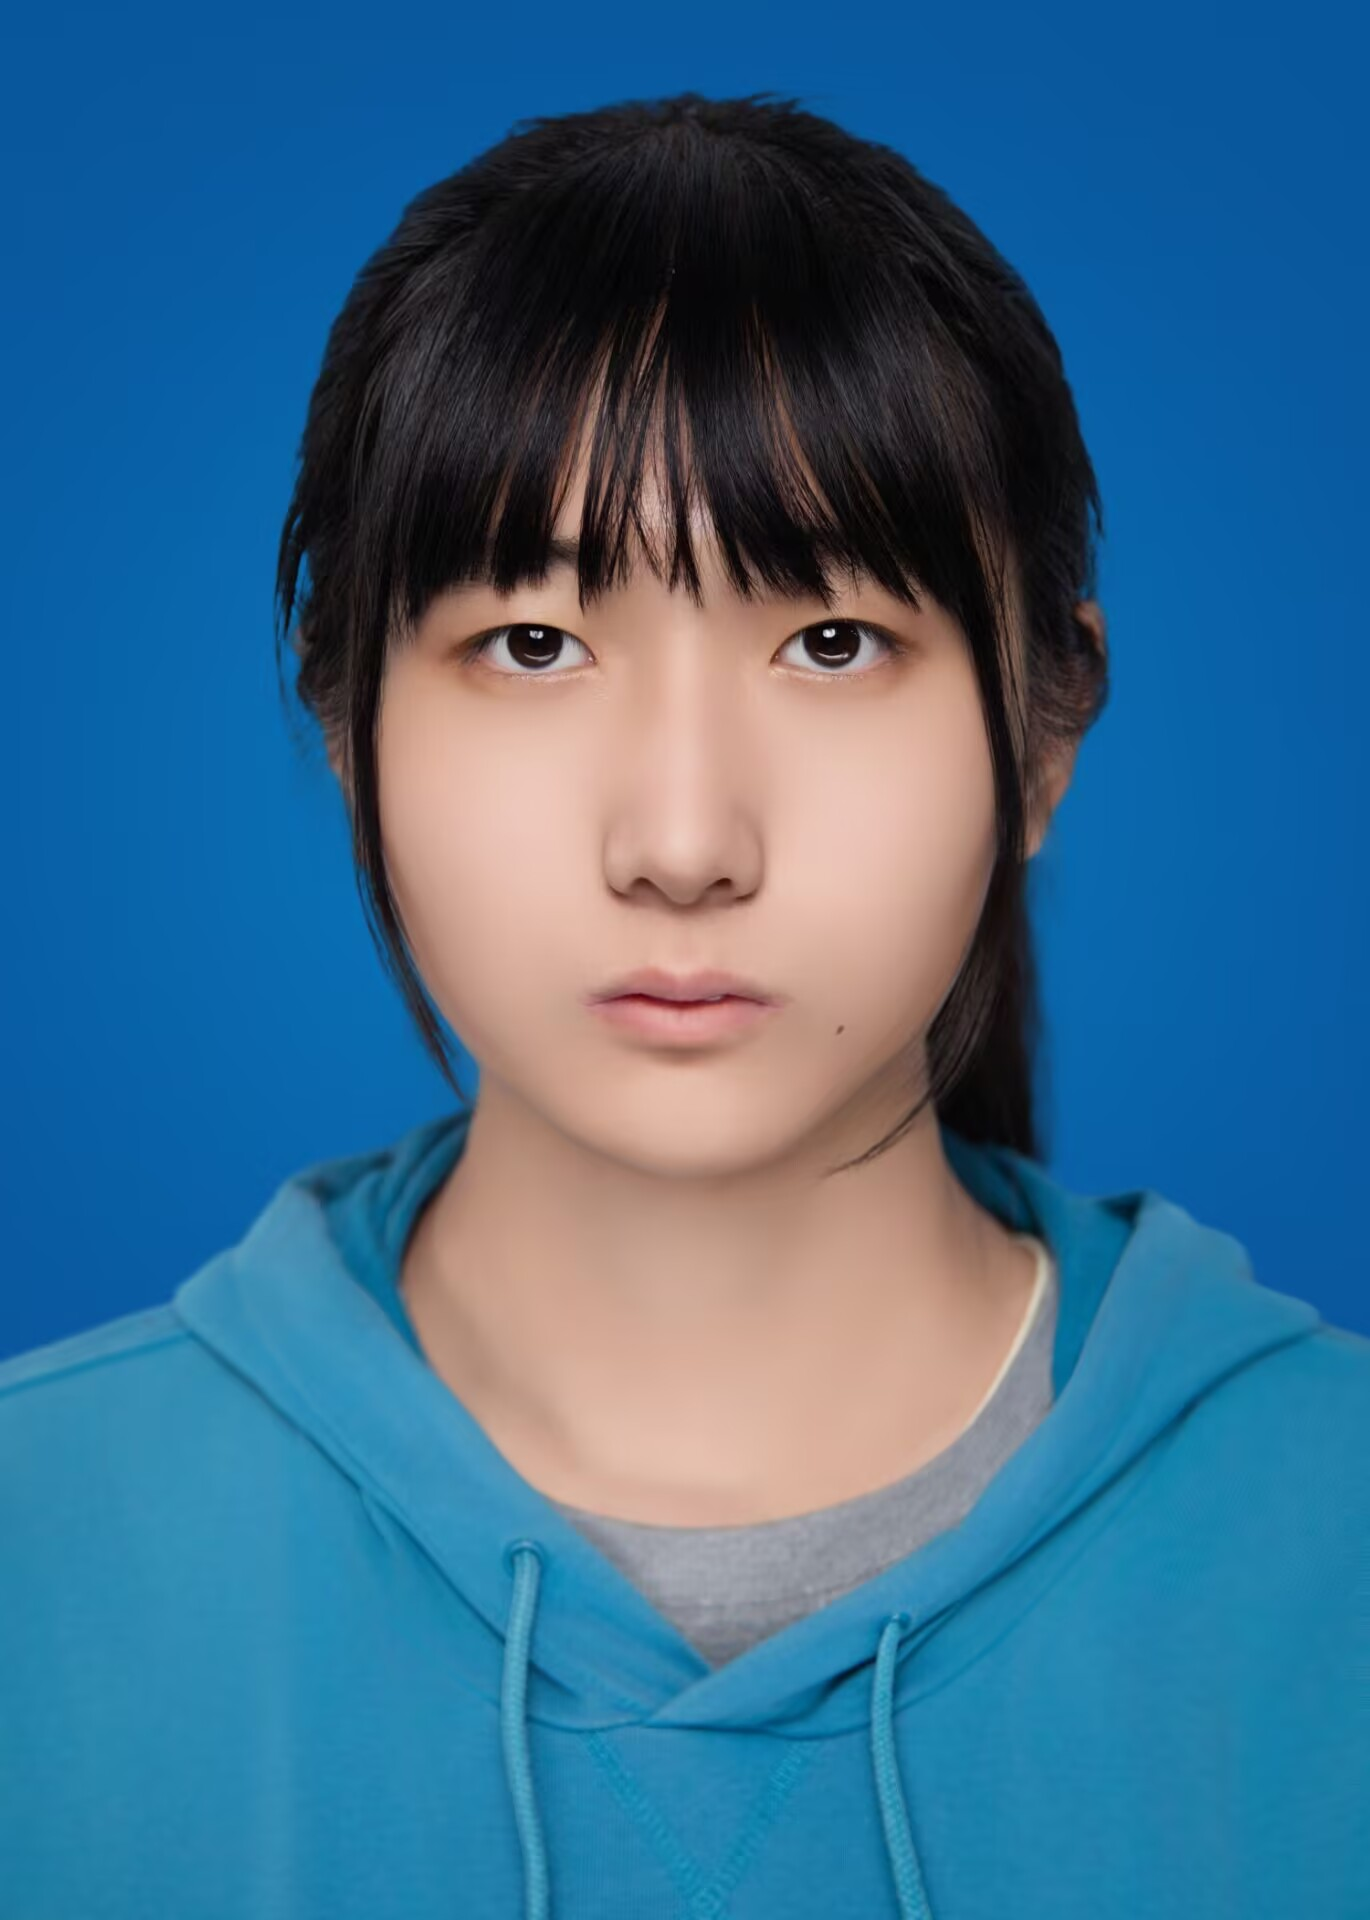
\includegraphics[width=0.2\textwidth]{Jin_Chenye.png} & He is a sophomore majoring in software engineering. He is highly accomplished in algorithms, artificial intelligence, and other software engineering skills. He has won many awards in algorithm competitions and artificial intelligence.He is one of the main responsible for the operation and maintenance of the GPU cluster in the school. \\
\hline
Li Wangyang & 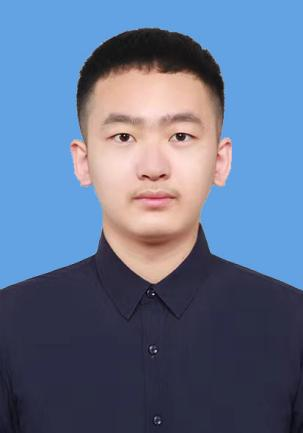
\includegraphics[width=0.2\textwidth]{Li_Wangyang.png} & He is a sophomore majoring in software engineering. He has made great achievements in the field of high performance computing and parallel computing. He is one of the main leaders of the GPU cluster operation and maintenance in the school, and has rich operation and maintenance experience. \\
\hline
Cui Shuyang & 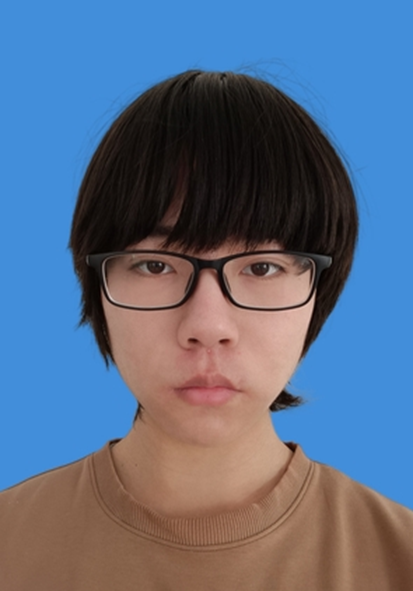
\includegraphics[width=0.2\textwidth]{Cui_Shuyang.png} & He is a sophomore majoring in software engineering. He specializes in high performance computing testing, parallel computing, artificial intelligence algorithms, etc. He is also one of the main heads of the GPU cluster operation and maintenance in the school. \\
\hline
Li Jinze & 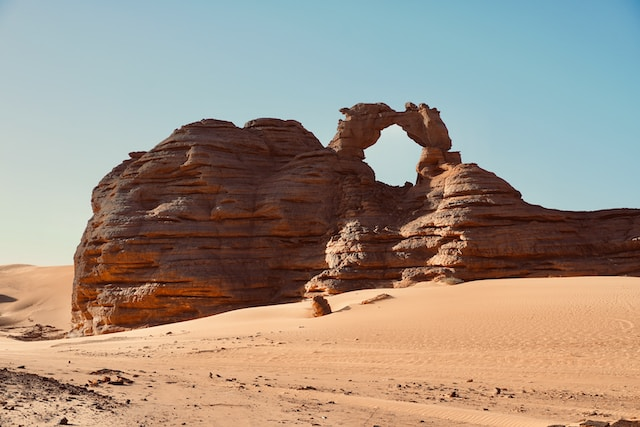
\includegraphics[width=0.2\textwidth]{Li_Jinze.png} & He is a senior majoring in software engineering. He specializes in high performance computing testing, parallel computing, and artificial intelligence algorithms. He is not only strong, but also has a wealth of experience in the competition, which is one of the core of this cmpetition. \\
\hline
Fang Yi & 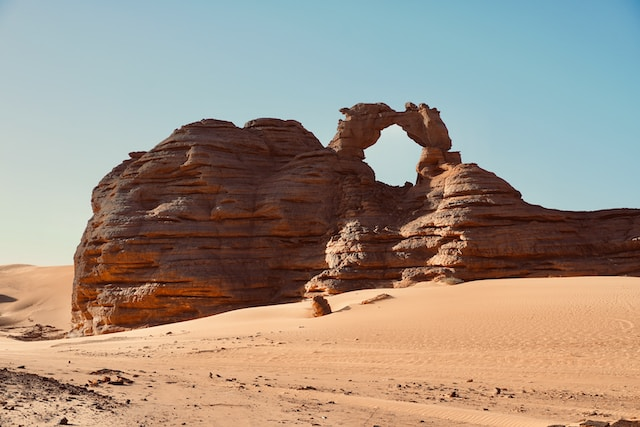
\includegraphics[width=0.2\textwidth]{Fang_Yi.png} & He is a sophomore in the software engineering department. He is good at algorithms and has a great interest in high performance computing and parallel computing. He kept learning and improving in this competition, and used his knowledge to solve problems. \\
\hline
\end{tabular}
\end{table}
\begin{figure}[H]
    \centering
    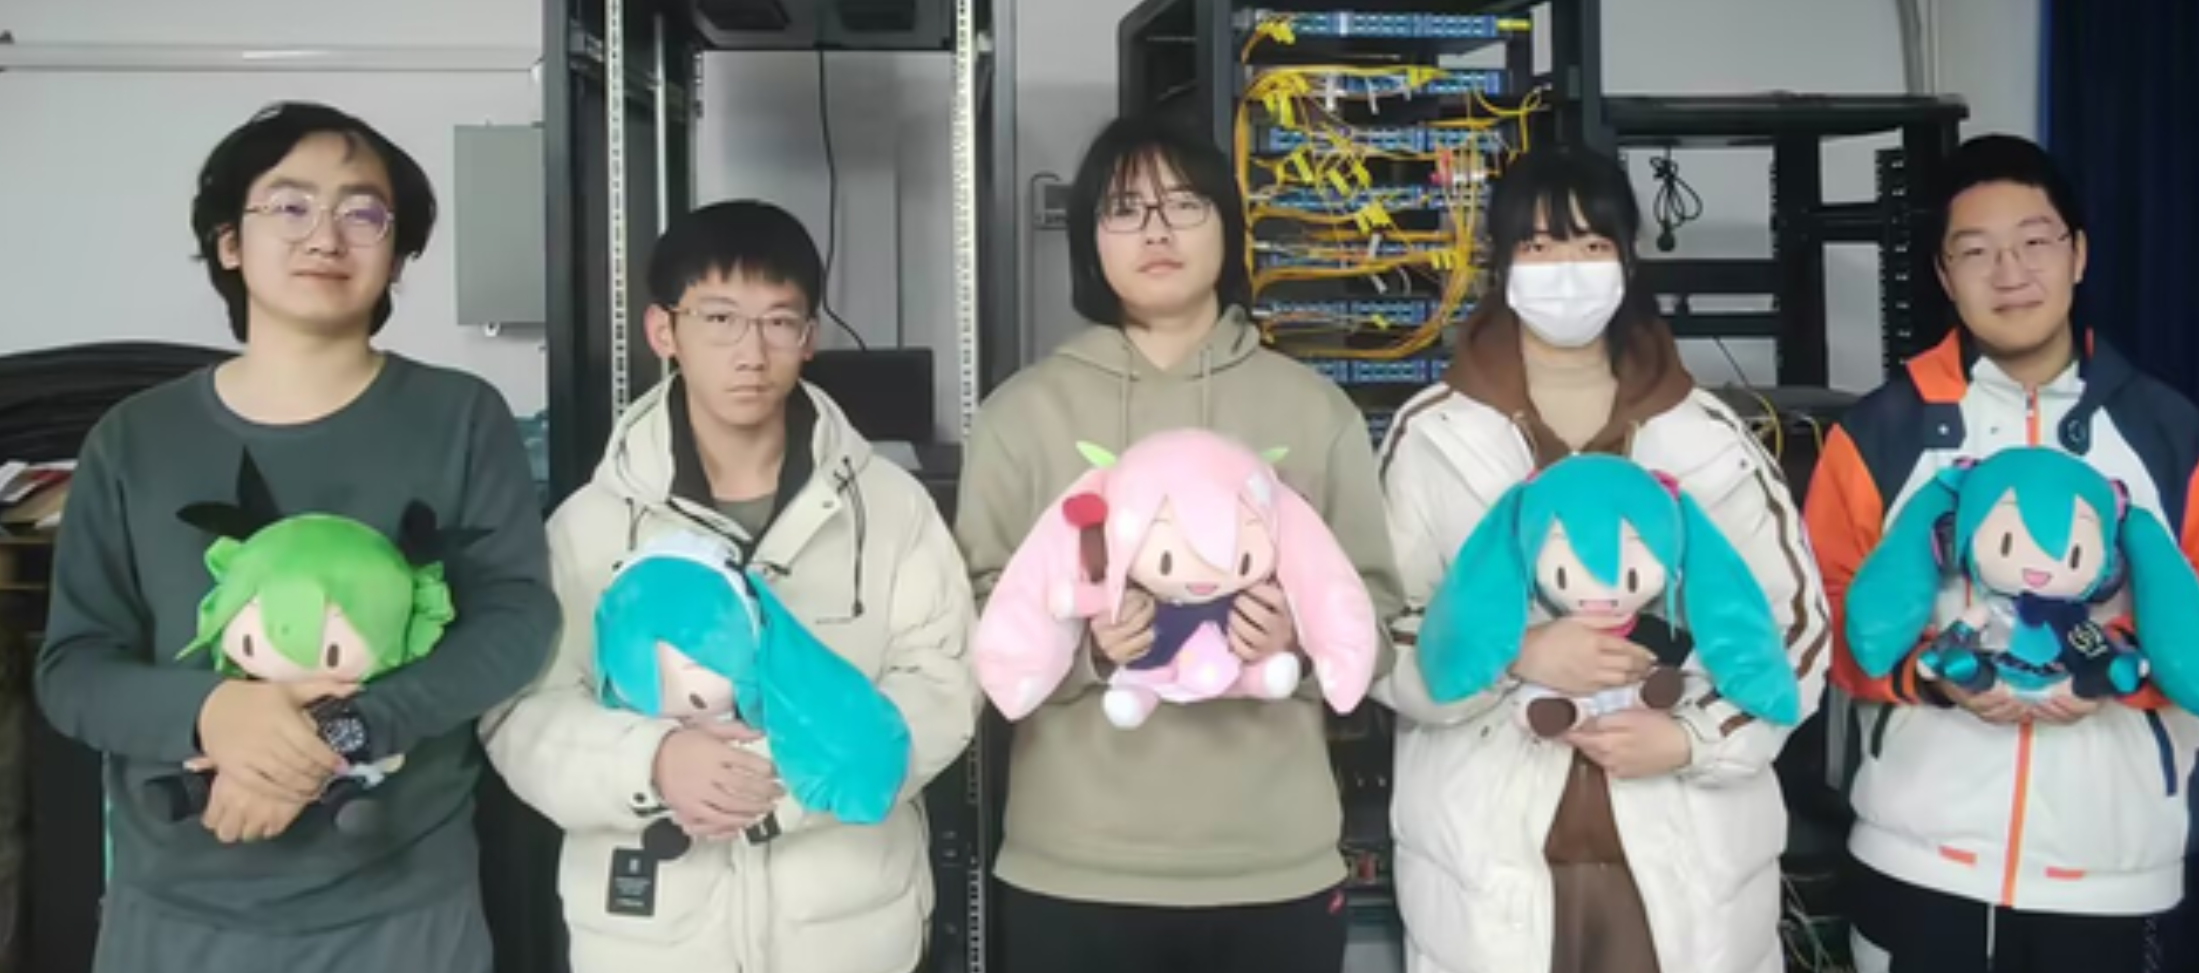
\includegraphics[width=0.8\textwidth]{Team_Photo.png}
    \caption{Team photo}
    \label{fig:team_photo}
\end{figure}


\subsection{Team Motto}
YSUers save the world.

\newpage

\section{Technical Proposal Requirements}

\subsection{Design of HPC System}

\subsubsection{Theoretical Design of an HPC Cluster}
To archive the goal of best computing performance within the limitation of 3KW power consumption, we designed 2 types of nodes in our cluster: CPU node and GPU node.
CPU node: each node contains 2 CPU.
GPU node: each node contains 2 CPU and some GPU.
Not all of those components are active during use, some of them will keep idle.

We designed a HPC system with a total of 4 nodes. Our estimated total system power consumption is less than 3KW when the system is running in both modes described below.
CPU mode: in this mode, the CPUs of all nodes work while the GPUs of the GPU nodes will remain idle. This computing mode is suitable for high-performance applications that run only on CPUs.
GPU mode: In this mode, CPU nodes are idle and GPU nodes work. This computing mode is suitable for applications that require computation on GPU.

\subsubsection{Software and Hardware Configurations}
The general single CPU node configuration is shown below:
\begin{table}[H]
\centering
\caption{Single Node Configuration}
\begin{tabular}{|l|l|l|}
\hline
Component Name & Model & Num \\
\hline
Server & Inspur NF5280M7 & 1 \\
\hline
CPU & Intel Xeon 6530 & 2 \\
\hline
Memory & DDR5 32G & 16 \\
\hline
HardDrive & SSD 480G & 1 \\
\hline
HCA & InfiniBand Mellanox ConnectX®-7 HDR & 1 \\
\hline
\end{tabular}
\end{table}

The configuration of CPU node 1 is the same as the single node configuration described above.GPU node 1 adds 1 NVIDIA H100 80G PCIe GPU on top of the CPU node 1 configuration, and GPU nodes 2,3 add 4 NVIDIA H100 80G PCIe GPUs on top of the single node configuration and replace the CPUs with Xeon 6538Y+.

\textbf{Node1 (CPU Node)}: General Node Configuration
\textbf{Node2 (Master GPU Node)}: General Node Configuration + 1 * H100 GPU
\textbf{Node3 (GPU Node)}: General Node Configuration + 2 * H100 GPU + 2 * Xeon 6538Y+
\textbf{Node4 (GPU Node)}: General Node Configuration + 2 * H100 GPU + 2 * Xeon 6538Y+

\subsubsection{Interconnection, Power Consumption, Performance Evaluation, and Architecture Analysis}
All nodes are connected via 1000M Ethernet and InfiniBand networks. Ethernet is used to transmit control data and InfiniBand provides high-speed inter-node interconnectivity. For two GPU nodes, the GPUs in the nodes are connected to each other via NVIDIA NVLink to provide high-speed interconnectivity between the GPUs.

\begin{figure}[H]
    \centering
    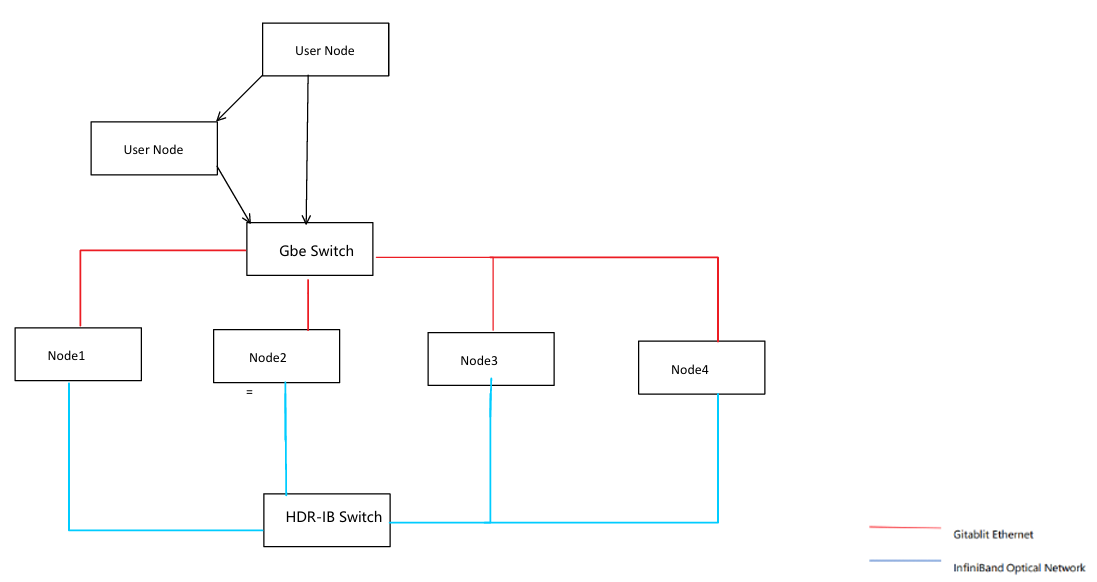
\includegraphics[width=0.6\textwidth]{Cluster_Architecture.png}
    \caption{Cluster Architecture}
    \label{fig:cluster_arch}
\end{figure}

\begin{table}[H]
\centering
\caption{Cluster software configuration}
\begin{tabular}{|l|l|}
\hline
Item & Version \\
\hline
OS & CentOS 7.9 \\
\hline
Compiler & GCC 10, Intel oneAPI BaseKit 2022.3.1(icc) \\
\hline
Math Library & Intel oneAPI MKL 2022.2 \\
\hline
MPI & Intel oneAPI HPCKit 2022.3.1 \\
\hline
Other & NVIDIA Data Center Driver for Linux RHEL 7 verson 535 \\
\hline
\end{tabular}
\end{table}

According to the power calculator on Inspur's official website, the power consumption of the predecessor NF5280M6 of the NF5280M7 server we used is shown in the table below:
\begin{table}[H]
\centering
\caption{NF5280M6 Power Consumption}
\begin{tabular}{|l|l|}
\hline
Loads & Power consumption \\
\hline
100\% & 695.88W \\
\hline
50\% & 433.00W \\
\hline
25\% & 304.15W \\
\hline
0\% & 177.68W \\
\hline
\end{tabular}
\end{table}

Therefore, after comparing the differences between the servers, we presume the power consumption of the CPU 1 node and the GPU 1 node (without the GPU) to be
\begin{table}[H]
\centering
\caption{NF5280M7 Power Consumption with Xeon 6538Y+}
\begin{tabular}{|l|l|}
\hline
Load & Power consumption \\
\hline
100\% & 670W \\
\hline
50\% & 410W \\
\hline
25\% & 285W \\
\hline
0\% & 150W \\
\hline
\end{tabular}
\end{table}

All node power consumption in the power consumption data below is assumed from the table above.

\textbf{CPU Mode:}

\textbf{GPU Mode:}
\begin{table}[H]
\centering
\caption{Power Consumption in GPU mode}
\begin{tabular}{|l|l|}
\hline
Component & Power consumption \\
\hline
4 Nodes & 2780W \\
\hline
InfiniBand Switch & 100W \\
\hline
Ethernet Switch & 20W \\
\hline
GPU(Idle) & 100W \\
\hline
Total Power & 3000W \\
\hline
\end{tabular}
\end{table}

We use Flops (floating point operations per second) to estimate the theoretical performance of the cluster.
The Xeon 6530 and 6530Y+ CPU has 2 FMA engines per core. Each FMA engine has 8 lanes and each lane can perform 2 floating point operations per cycle. In this way, we estimate the theoretical performance to be:
\begin{equation*}
2FMA \times 8lanes \times 2Flopspercycle \times 32cores \times 2sockets \times 4nodes \times 2.6GHz = 21299.2 GFlops = 21.2992 TFlops
\end{equation*}
n GPU mode, the floating-point performance of a single H100 card is 51.22 TFlops, so the floating-point performance of the entire cluster is:
\begin{equation*}
51.22TFlops \times 5 = 256.1 TFlops
\end{equation*}

\begin{table}[H]
\centering
\caption{Cluster Performance}
\begin{tabular}{|l|l|}
\hline
Mode & Performance \\
\hline
CPU & 21.2922 TFlops \\
\hline
GPU & 256.1 TFlops \\
\hline
\end{tabular}
\end{table}

During the formation of the cluster, we used the server power calculation tool provided by Inspur to more accurately estimate power consumption. The cluster uses InfiniBand, a high-performance communication technology protocol with lower latency, greater bandwidth, and higher reliability for more powerful I/O performance, which is ideal for high-speed interconnection of nodes in a cluster. In addition, we have introduced NVLink technology in GPU nodes. NVLink technology provide high-speed interconnections between GPUs and CPUs for NVIDIA H100 graphics cards, and it is more than seven times faster than PCIe bandwidth compared to traditional PCIe links. This also makes it ideal for GPU-intensive high-performance computing. However, the cluster we built still has some shortcomings. At the software level, we did not use the latest packages (e.g., we used Intel oneAPI 2022 instead of 2023), which introduces support for new architectures but can also lead to compatibility issues, as was the case with some of the questions in the ASC competition. Also, at the hardware level, the H100 GPUs we used do not perform optimally in this power constraint and network topology, which is more noticeable when performing scenarios that require multi-card collaboration such as LLM training.

\subsection{HPL and HPCG Benchmarks}

\subsubsection{Software Environment}
\begin{table}[H]
\centering
\caption{Hardware Configuration}
\begin{tabular}{|l|l|}
\hline
Item & Configuration \\
\hline
CPU & Intel Xeon Gold 5218R x2 \\
\hline
Memory & DDR3 128GB \\
\hline
\end{tabular}
\end{table}

\begin{table}[H]
\centering
\caption{Software Configuration}
\begin{tabular}{|l|l|}
\hline
Item & Configuration \\
\hline
OS & CentOS 7.9.2009 \\
\hline
Compiler & Intel mpiicc 2021.11 \\
\hline
Math Library & Intel Math Kernel Library 2024.0 \\
\hline
MPI & Intel MPI Library 2021.11 \\
\hline
\end{tabular}
\end{table}


\subsubsection{Performance Optimization and Testing Methods}
\textbf{2.2 HPL}

\textbf{2.2.1 Background}
HPL is a software package that solves a (random) dense linear system using double precision (64 bits) arithmetic on distributed-memory computers. It is a portable and free implementation of the High Performance Computing Linpack Benchmark.
The HPL package includes a testing and timing program that measures the accuracy and speed of the solution. The performance of this software on your system depends on many factors. However, with some assumptions on the interconnection network, the algorithm and its implementation described here are scalable, meaning that their parallel efficiency remains constant with the per processor memory usage.

\textbf{2.2.2 Test Principle}
When the matrix size is N, time of floating point arithmetic is:
\begin{equation*}
3/2 \times N \times N \times N - 2 \times N \times N
\end{equation*}
Therefore, as the problem size N is given, and the time T of system calculation is measured, the system performance can be estimated according to the following formula (unit flops, number of floating point arithmetic completed per second)
\begin{equation*}
performance = number/time = (3/2 \times N \times N \times N - 2 \times N \times N) / T
\end{equation*}

\textbf{2.2.3 HPL Algorithm Analysis}
The algorithm used by HPL can be summarized by the following keywords: Two-dimensional block-cyclic data distribution - Right-looking variant of the LU factorization with row partial pivoting featuring multiple look-ahead depths Recursive panel factorization with pivot search and column broadcast combined - Various virtual panel broadcast topologies bandwidth reducing swap-broadcast algorithm backward substitution with look-ahead of depth.

\textbf{(1) LU decomposition}
Firstly, HPL compute the LU factorization of matrix A
\begin{equation*}
LU=A
\end{equation*}
L is the lower triangular matrix, is the upper triangular matrix
\begin{equation*}
Ax=(LU) \cdot x=L \cdot (U \cdot x)=b
\end{equation*}
Solve for the y vector
\begin{equation*}
Ly=b
\end{equation*}
And then solve for x
\begin{equation*}
U x=y
\end{equation*}
So for Ax is equal to b, can convert Ax is equal to b into an upper trigonometric system. LU factorization of the matrix (A,b) to get the upper triangular matrix. The LU decomposition process is shown in the figure below:

\begin{figure}[H]
    \centering
    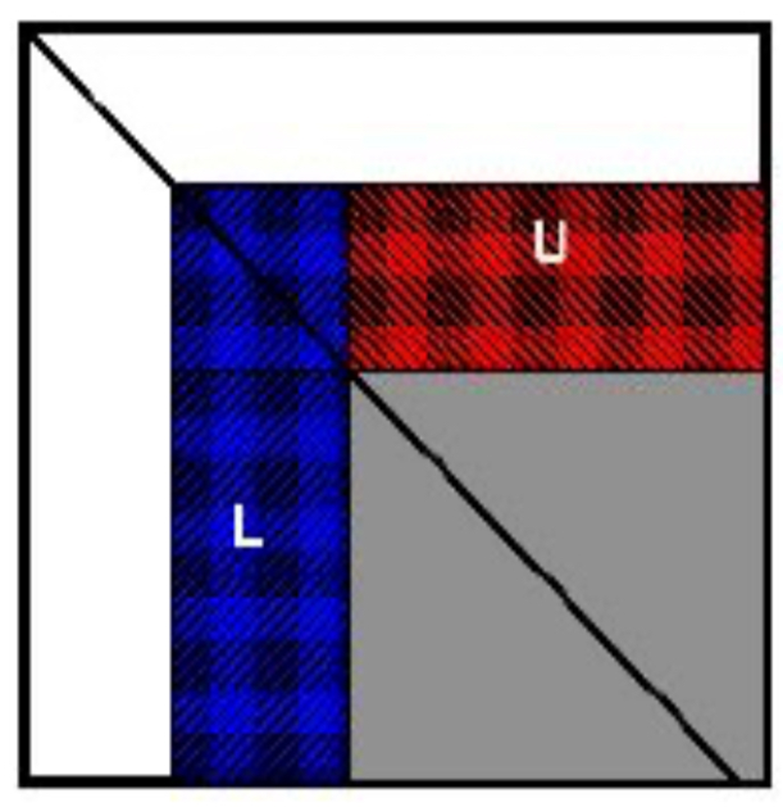
\includegraphics[width=0.7\textwidth]{LU_factorization.png}
    \caption{LU factorization}
    \label{fig:lu_factorization}
\end{figure}

\begin{figure}[H]
    \centering
    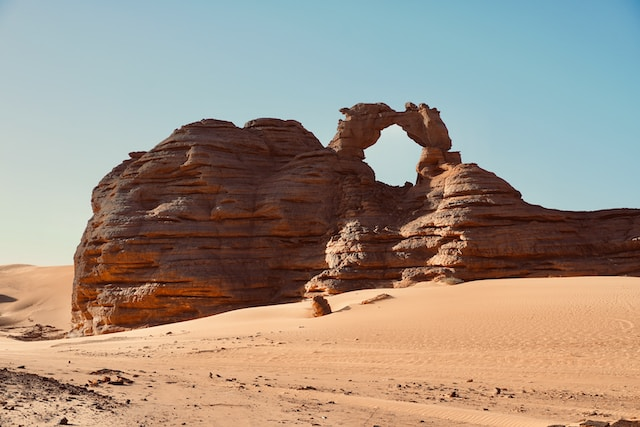
\includegraphics[width=0.7\textwidth]{LU_decomposition_process.png}
    \caption{LU decomposition process}
    \label{fig:lu_decomposition}
\end{figure}

First complete the decomposition of $A_{11}$, then complete the decomposition of $A_{12}$and $A_{22}$, finally update$A_{22}$. According to such a calculation sequence, the two-dimensional block-cyclic data distribution strategy needs to be adopted to divide the data of the matrix to each process in parallel LU decomposition.

\textbf{(2)Block Cyclic Data Distribution}
The Block Cyclic Data Distribution strategy is step-wise to a 2D GRID of P X Q processes to ensure load balancing and scalability of the algorithm. NB is the width of the panel. And the data in the process are stored continuously. Interprocess data distribution is shown in the figure below:

\begin{figure}[H]
    \centering
    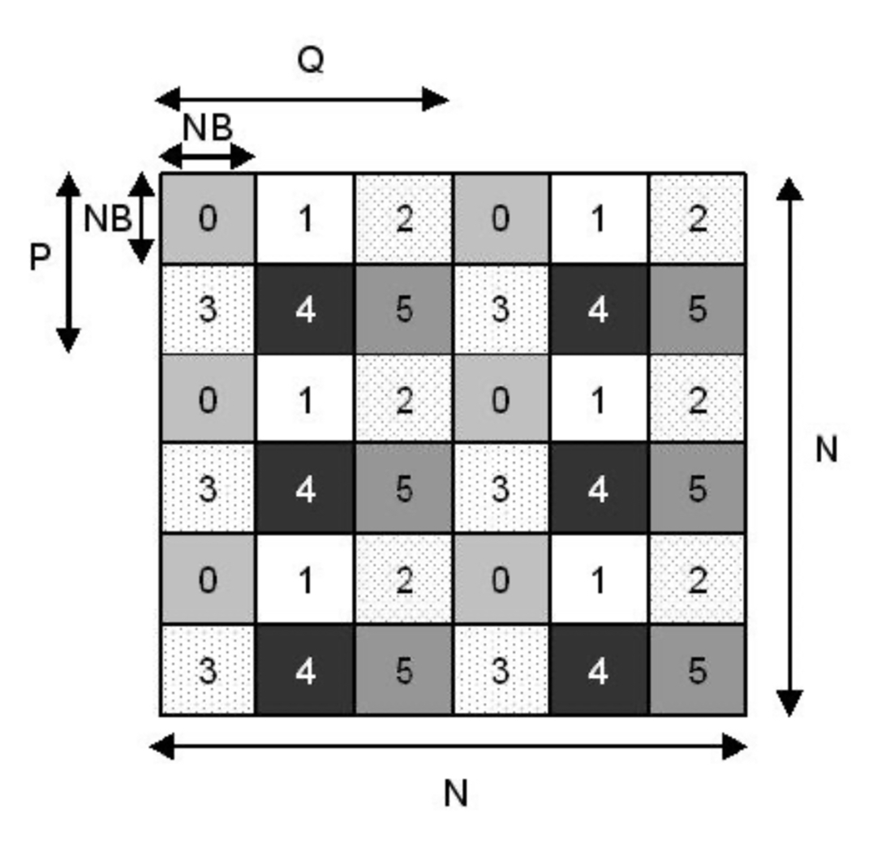
\includegraphics[width=0.7\textwidth]{Interprocess_data_distribution.png}
    \caption{Interprocess data distribution}
    \label{fig:interprocess_data}
\end{figure}

The way the matrix is distributed on the process has a great influence on the load balancing and communication characteristics of the concurrent algorithm and therefore determines its performance and scalability to a large extent. Circular block distribution provides a simple and general method for distributing block partitioning matrices on distributed memory concurrent computers. The block cycle data distribution is determined by four parameters P,q, and m,n, where P,q is the process grid M and N determines the block size. Blocks separated by fixed strides in column and row directions are assigned to the same processes.

\textbf{(3).Panel broadcast}
For process grid with multiple columns, every cycle is calculated only a list of the panel process execution decomposition, decomposition of the panel process to perform a panel of each column line communication exchange algorithm and choose the maximum principal yuan, panel decomposition calculation, after the completion of the decomposed data broadcast to other processes, swapping operation lines (exchange and radio), Each process saves a copy of the current U matrix and updates the trailing matrix with the latest Panel and U. The calculation process is shown in the figure below:

\begin{figure}[H]
    \centering
    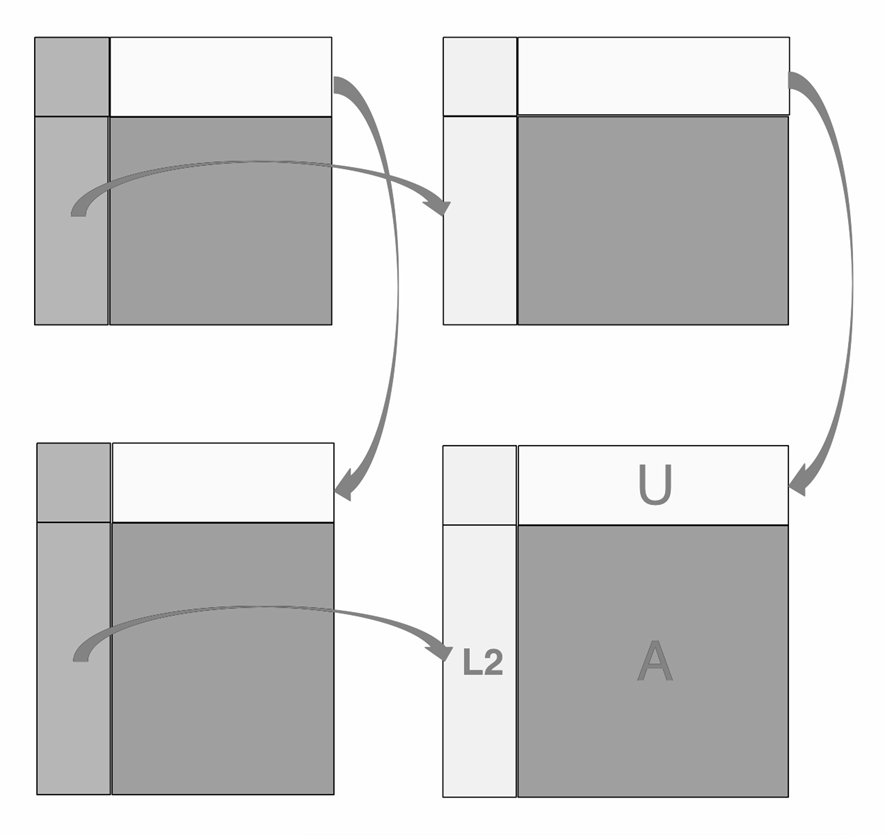
\includegraphics[width=0.7\textwidth]{Panel_broadcast_process.png}
    \caption{Panel broadcast process}
    \label{fig:panel_broadcast}
\end{figure}

\textbf{(4).Panel decomposition}
Panel decomposition is completed by a row of processes that currently have this Panel block. Each time, the largest principal element is selected, an element in the first line of the Panel is exchanged, and the row where the largest principal element is broadcast to each process, and the first number is solved by each process.
In the process of selecting the maximum principal element, each process selects the row where the maximum principal element is and copies it to the buffer. After two pairs are exchanged, each process selects the row where the maximum principal element is and puts it in the buffer.

HPL adopts the row principal element algorithm. Before the single-step matrix update, the largest rows selected by panel decomposition should be exchanged into THE U matrix, and the row principal element exchange and broadcast of the un-updated matrix should be performed. After that, each process obtains the complete number of main element rows. Each process on each column selects the result of the maximum principal element for the row exchange operation. There are NB maximum principal elements in the matrix, which exchange with data in U in turn.

In the panel decomposition stage, subscripts and the process where the data to be exchanged have been calculated and sent to each process along with panel broadcast.

\textbf{2.2.4Parameter Settings}

\textbf{2.2.4.1Size of Matrix}
N represents the number and scale of matrices to be solved.The larger the matrix size n is,the greater the proportion of effective calculation, The higher the floating-point processing performance of the system.

\begin{figure}[H]
    \centering
    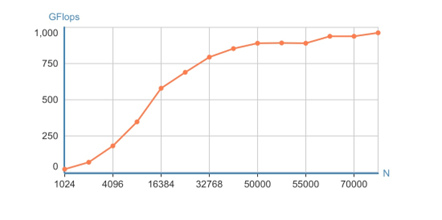
\includegraphics[width=0.7\textwidth]{GFLOPS_N.png}
    \caption{GFLOPS with different input of N}
    \label{fig:gflops_n}
\end{figure}

However, the increase of matrix size will lead to the increase of memory consumption, If the actual memory space of the system is insufficient,using swap partitions,Performance will be greatly reduced. The matrix occupies about 80\% (or 90\%) of the total memory of the system, that is:
\begin{equation*}
N \times N \times 8bytes = memory \times 80\%
\end{equation*}
Therefore, when the value of n is 113137, the effective calculation accounts for a high proportion.

\textbf{2.2.4.2 Size of Block Matrix}
NB is the size of the matrix block. In the process of solving the matrix, the size of the matrix block has a great impact on the performance. The choice of NB is closely related to many factors of software and hardware. The selection of Nb value generally follows the following rules:
\begin{itemize}
    \item NB cannot be too large or too small, generally less than 384.
    \item NB x 8 must be a multiple of the cache line.
    \item The size of NB is related to communication mode, matrix scale, network, processor speed, etc.
    \item NB should be able to divide N.
\end{itemize}
According to the above rulestest we tried several NBs, the results are shown in the figure below.

\begin{figure}[H]
    \centering
    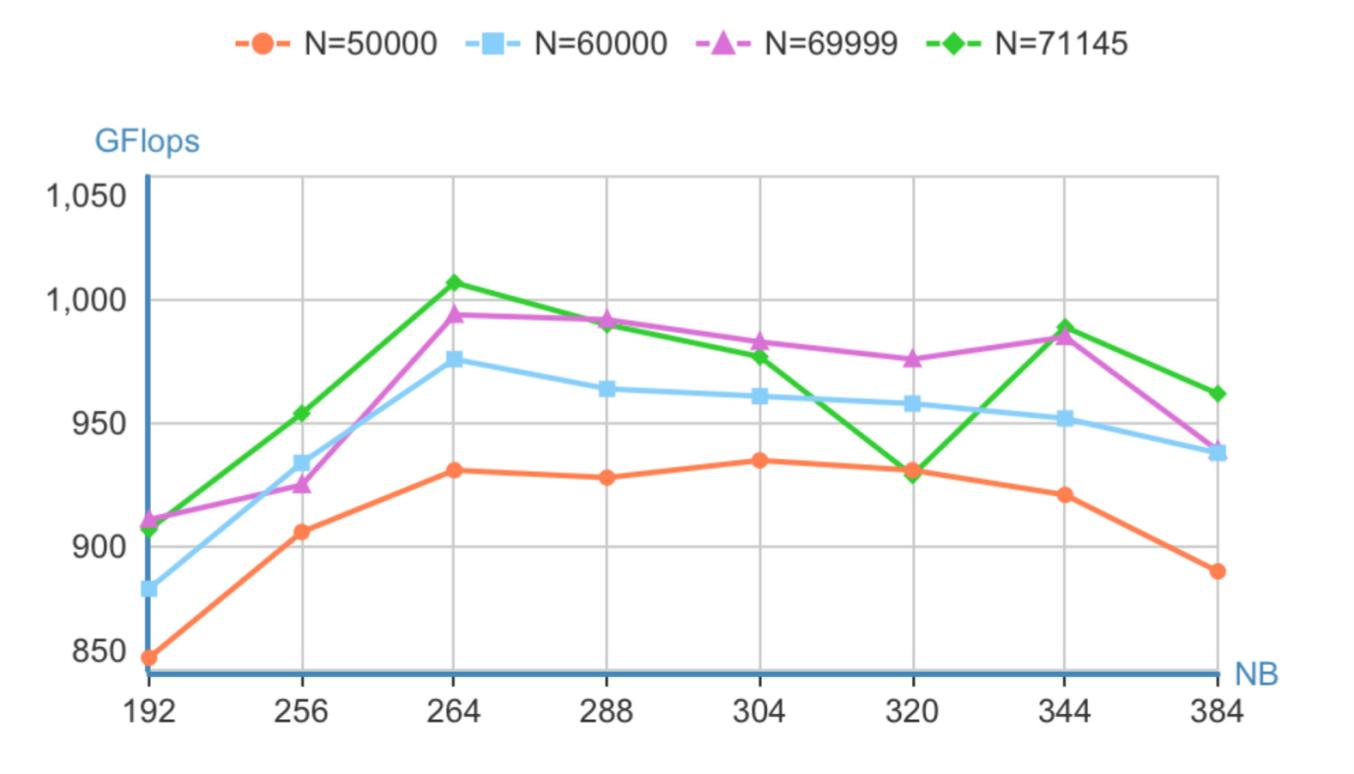
\includegraphics[width=0.7\textwidth]{GFLOPS_NB.png}
    \caption{GFLOPS with different input of N and NB}
    \label{fig:gflops_nb}
\end{figure}

It can be seen that when NB is around 264 or 344, the performance is better in our machine when N is bigger than 50000. As for 113137, we will try more NBs later.

\textbf{2.2.4.3Parameters of P and Q}
PxQ represents a two-dimensional processor grid where p represents the number of processors in the horizontal direction, Q indicates the number of processors in the vertical direction. Generally, one process corresponds to one CPU, with better performance. There is the following formula:
\begin{equation*}
P \times Q = number\ of\ cpu = number\ of\ process
\end{equation*}
We have 40 processors in total, so we tried several pairs of P and Q and make sure that their product is above 40. The results are shown in the figure below.

\begin{figure}[H]
    \centering
    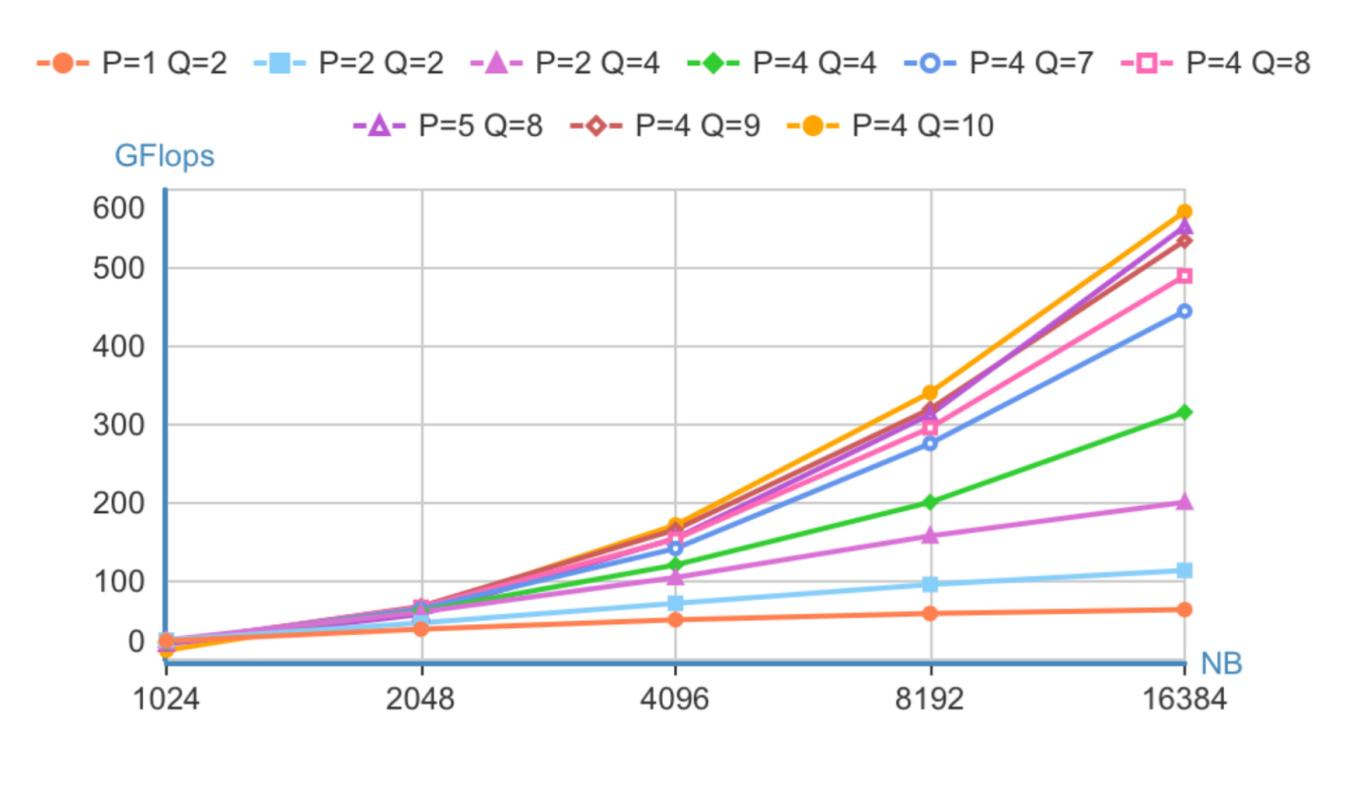
\includegraphics[width=0.7\textwidth]{GFLOPS_PQ.png}
    \caption{GFLOPS with different input of P and Q}
    \label{fig:gflops_pq}
\end{figure}

It is found that the performance is better when P is 4 and Q is 10. P=5 and Q=8 is also a good choice.

\textbf{2.2.5HPL Performance Evaluation}
Due to the limitation of objective conditions, HPL test is only conducted at a single computing node without GPU acceleration. The peak value of theoretical double precision floating-point calculation is as follows:
\begin{equation*}
Peak = 2 \times 20 \times 2.1GHz \times 16Flops/cycle = 1344Glops
\end{equation*}
And we tested several groups of parameters. The results are shown in the figure below.

\begin{figure}[H]
    \centering
    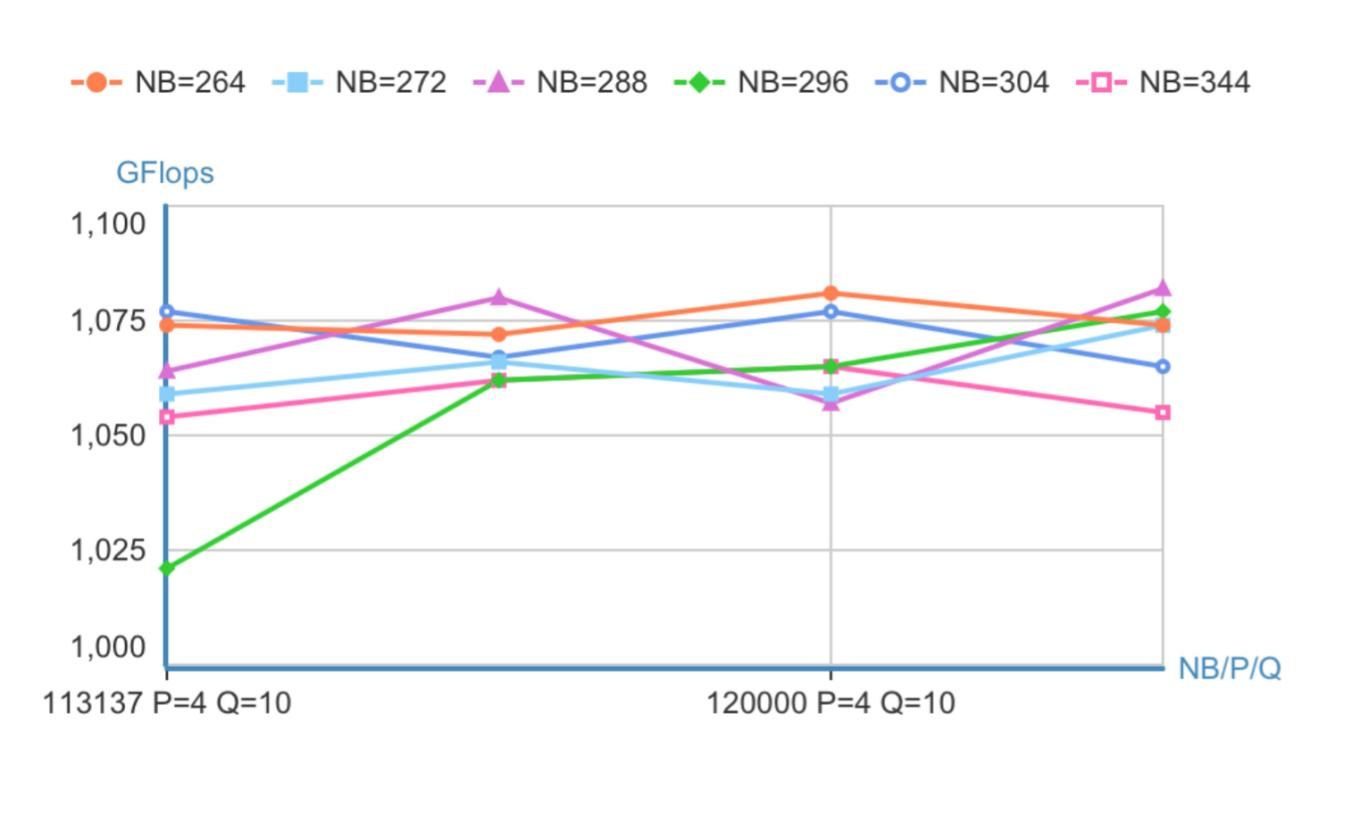
\includegraphics[width=0.7\textwidth]{GFLOPS_PQ_NB.png}
    \caption{GFLOPS with different input of P and Q}
    \label{fig:gflops_pq_nb}
\end{figure}

Finally, the best parameter settings obtained through the test are as follows:
\begin{table}[H]
\centering
\caption{Parameter settings}
\begin{tabular}{|l|l|l|l|}
\hline
N & NB & P & Q \\
\hline
120000 & 288 & 5 & 8 \\
\hline
\end{tabular}
\end{table}

The actual double precision floating-point calculation peak obtained from the above parameter test is 803.698 GFlops. Therefore, the final HPL calculation efficiency is:
\begin{equation*}
Performance-Ratio = 1082.5Gflops/1344Gflops = 80.54\%
\end{equation*}

\textbf{2.2.6Document introduction}
\begin{itemize}
    \item (1)hpl\_N\_NB.out and hpl\_N\_NB\_2.out: The output with different Ns and NBs. We choose N and NB according it.
    \item (2)hpl\_N\_PQ.out: The output with different pairs of P and Q. We choose P and Q according it.
    \item (3)hpl.out: The final test output, which including the peek performance we got.
\end{itemize}

\textbf{2.3 HPCG}

\textbf{2.3.1 Background}
The High Performance Conjugate Gradients (HPCG) Benchmark project is an effort to create a new metric for ranking HPC systems. HPCG is intended as a complement to the High Performance LINPACK (HPL) benchmark, currently used to rank the TOP500 computing systems. The computational and data access patterns of HPL are still representative of some important scalable applications, but not all. HPCG is designed to exercise computational and data access patterns that more closely match a different and broad set of important applications, and to give incentive to computer system designers to invest in capabilities that will have impact on the collective performance of these applications.

Compared with the HPL benchmark test, its calculation, memory access and communication modes are more representative of a wide range of scientific and engineering computing applications, which based on partial differential equation solving. Also, it helps to reflect the system's memory access bandwidth, latency and communication energy more comprehensively, to make up for the deficiencies and drawbacks of the hpl test. But the test results are usually lower than the HPL test results, often only have a few percent.

\textbf{2.3.2 Test Principle}
In a large-scale parallel environment, HPCG uses a three-dimensional area decomposition strategy, which is to divide the entire computing area into sub-areas according to 3 dimensions,and then each sub-areas is assigned an MPI process. The HPCG program includes dot product (DDOT), vector update function (Waxpby), large sparse matrix multiplication (SYMV) and triple solver (SYMGS) and Multi-Grid algorithm (MG).

\begin{figure}[H]
    \centering
    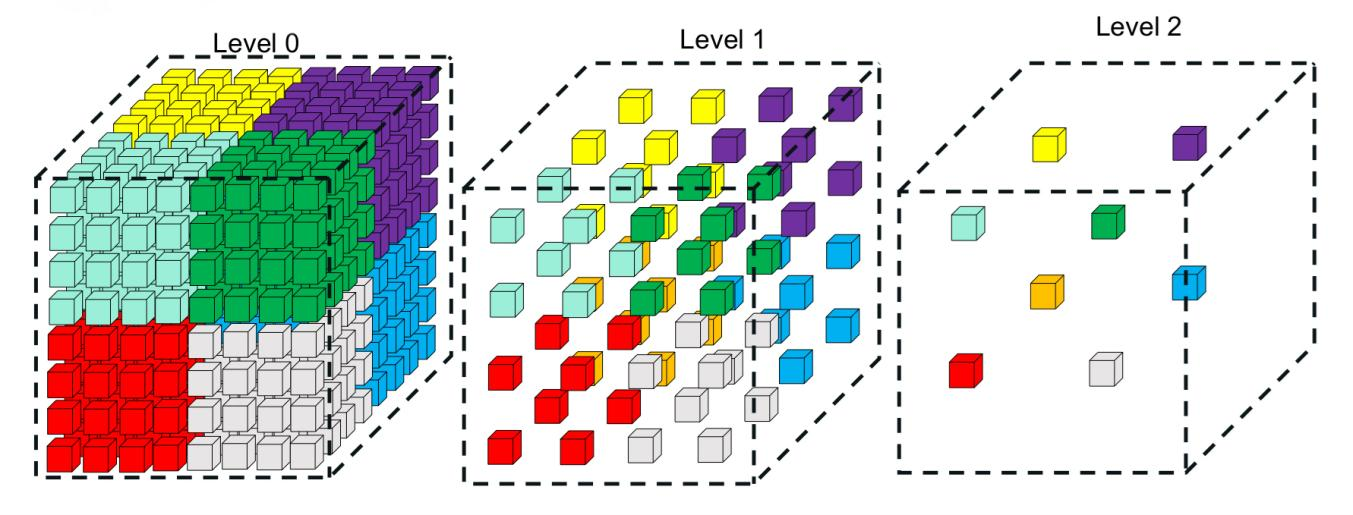
\includegraphics[width=0.7\textwidth]{SYMGS_restriction_process.png}
    \caption{SYMGS restriction process}
    \label{fig:symgs_restriction}
\end{figure}

\textbf{2.3.3Build HPCG}
We used both intel oneAPI Tools and GCC to compile it. After test, we found that the hpcg program with intel compiler performed better on our intel Xeon processors. So we chose the ICPC\_OMP arch.

\textbf{2.3.4Parameter Settings}

\textbf{2.3.4.1Testing Time}
HPCG can be run in just a few minutes from start to finish. However, official runs must be at least 1800 seconds (30 minutes) as reported in the output file. To achieve a balance between validity and efficiency, and make sure that the valid run time is more than 1800 seconds, we took 3600s as the run time of HPCG, which is able to get a valid result with acceptable time consumption.

\textbf{2.3.4.2Problem Size}
A valid run must also execute a problem size that is large enough so that data arrays accessed in the CG iteration loop do not fit in the cache of the device in a way that 21 would be unrealistic in a real application setting. Presently this restriction means that the problem size should be large enough to occupy a significant fraction of “main memory”, at least 1/4 of the total. Based on this rule, We choose several problem sizes, trying to make out which can lead to best performance.
The parameter local domain dimension specified by user in hpcg.dat predicts the problem size. The default local domain dimension is 192 × 192 × 192. Higher performance is observed when small problem size is specified. However, values under 32 will be defaulted to 32(for a 32x32×32 mesh). Therefore, we choose 32 as the local domain dimension.

\textbf{2.3.5Performance Estimation}
Performance ratio of HPL test value and theoretical peak value:
\begin{equation*}
Performance-Ratio = 1344Gflops/10.8092Gflops = 0.804\%
\end{equation*}
Performance ratio of HPL test value and HPCG test value:
\begin{equation*}
Performance-Ratio = 1082.5Gflops/10.8092Gflops = 0.998\%
\end{equation*}

\textbf{2.3.6Document introduction}
\begin{itemize}
    \item (1)HPCG-Benchmark.txt: the final output of HPCG test.
\end{itemize}


\subsection{Optimization for AlphaFold3 Inference}

\subsection{GPU Inference Optimization}

\subsubsection{Model Deployment}
Since the program requires more than 18GB of video memory, we chose to deploy the model on the YSU HPC supercomputing cluster. Dependencies were installed according to the official dockerfile documentation. Due to the cluster's CUDA driver version being 12.0, which differs from the dockerfile's 12.6, we needed to select a different jax version. According to the \href{https://docs.jax.dev/en/latest/installation.html#nvidia-gpu}{jax installation documentation}, we used the following commands to install jax:

\begin{lstlisting}[language=bash]
pip install --upgrade pip
pip install --upgrade "jax[cuda12]"
\end{lstlisting}

After installation, the jax version is 0.5.0, which differs from the version required in the dockerfile but still runs normally.

\subsubsection{Hardware Configuration}
Using the compute01 node of the supercomputing cluster, which is configured with: CPU: Intel Xeon Gold 5218R @ 2.10GHz, GPU: 2* NVIDIA GeForce 3090 24G, RAM: 125G.

\subsubsection{Environment Variables Setup}
\begin{lstlisting}[language=bash]
export XLA_PYTHON_CLIENT_MEM_FRACTION=0.95
export JAX_TRACEBACK_FILTERING=off
\end{lstlisting}

\subsubsection{Program Execution Command}
\begin{lstlisting}[language=bash]
python ./run_alphafold.py \
? --input_dir=/input_dir \
? --output_dir=/output_dir \
? --model_dir=/model_dir \
? --norun_data_pipeline \
? --num_recycles=3 \
? --flash_attention_implementation=xla
\end{lstlisting}

\subsubsection{Program Results}
See cluster files for details.

\subsection{Program Optimization}

\subsubsection{Optimization Strategy Overview}
Through code analysis and observation of program execution results, we found that the model inference phase accounts for over 95\% of the total runtime. Therefore, we prioritized optimizing the model inference time. Additionally, we identified optimization opportunities in the feature extraction phase.

\subsubsection{Optimization Methods}
\textbf{Model Inference Phase:} Used jax compilation cache directory to cache compiled functions and model parameters, reducing compilation time during model inference. \\
\textbf{Feature Extraction Phase:} Defined \texttt{FeatureCache} class to cache feature data, reducing repeated computations and memory usage. Implemented \texttt{optimize\_features} function to optimize data types and memory layout, \texttt{compress\_features} function to compress feature data, and parallel processing of feature data to reduce runtime.

\subsubsection{Optimization Methods}
Defined \texttt{create\_model\_runner} function to configure jax environment, including disabling 64-bit operations and setting thread count. Implemented \texttt{\_post\_process\_result} function for optimizing result processing and data type conversion. Created \texttt{ModelRunner} class with \texttt{\_split\_batch}, \texttt{run\_inference}, and \texttt{\_merge\_results} functions for dynamic batch processing, parallel model inference, and parallel result merging. Implemented \texttt{NumericsHandler} class with \texttt{handle\_coordinate\_numerics}, \texttt{handle\_general\_numerics}, and \texttt{check\_output\_numerics} functions for detecting and handling NaN/Inf values. Developed \texttt{CacheManager} class with \texttt{\_get\_cache\_key}, \texttt{\_serialize\_value}, \texttt{\_deserialize\_value}, and \texttt{put} functions for cache management. Created \texttt{MemoryManager} class with \texttt{get\_memory\_usage}, \texttt{update}, \texttt{cleanup}, and \texttt{monitor} functions for memory management.

\subsubsection{Optimization Results}
\textbf{Before optimization:} Total runtime: 3651.96s, Model inference: 3353.36s, Feature extraction: 298.60s. \\
\textbf{After optimization:} Total runtime: 3149.68s, Model inference: 3042.80s, Feature extraction: 106.88s. \\
\textbf{Total improvement:} 13.7\%, Model inference improvement: 9.3\%, Feature extraction improvement: 66.9\%.

\subsection{CPU Inference Optimization}

\subsubsection{Model Deployment}
Since the CPU version requires over 100GB of memory for large inputs, we chose to deploy the model on the login node of the YSU HPC supercomputing cluster, with the same deployment process as the GPU version.

\subsubsection{Hardware Configuration}
Using the login node configured with: CPU: Intel Xeon Gold 5218R @ 2.10GHz, RAM: 125G.

\subsubsection{Environment Variables Setup}
\begin{lstlisting}[language=bash]
export MKL_DEBUG_CPU_TYPE=5
export MKL_ENABLE_INSTRUCTIONS=AVX2
export KMP_AFFINITY="granularity=fine,compact,1,0"
export MKL_DYNAMIC=FALSE
\end{lstlisting}
\begin{lstlisting}[language=python]
import os
os.environ['JAX_PLATFORMS'] = 'cpu'
os.environ['JAX_SKIP_ROCM_TESTS'] = '1'
os.environ['JAX_SKIP_TPU_TESTS'] = '1'
os.environ['JAX_LOG_COMPILES'] = '0'
os.environ['TF_CPP_MIN_LOG_LEVEL'] = '3'
\end{lstlisting}

\subsubsection{Program Execution Command}
Same as GPU version.

\subsubsection{Program Results}
See cluster files for details.

\subsection{Program Optimization}

\subsubsection{Optimization Strategy Overview}
Through code analysis, we identified optimization opportunities in memory usage and CPU communication. We also found NaN/Inf values during program execution that needed handling.

\subsubsection{Optimization Methods}
Defined create\_model\_runner function to configure jax environment, including disabling 64-bit operations and setting thread count. Implemented \_post\_process\_result function for optimizing result processing and data type conversion. Created ModelRunner class with \_split\_batch, run\_inference, and \_merge\_results functions for dynamic batch processing, parallel model inference, and parallel result merging. Implemented NumericsHandler class with handle\_coordinate\_numerics, handle\_general\_numerics, and check\_output\_numerics functions for detecting and handling NaN/Inf values. Developed CacheManager class with \_get\_cache\_key, \_serialize\_value, \_deserialize\_value, and put functions for cache management. Created MemoryManager class with get\_memory\_usage, update, cleanup, and monitor functions for memory management.

\subsubsection{Optimization Results}
Before optimization: Total runtime: 44102.1s
After optimization: Total runtime: 43929.5s
Total improvement: 0.4\%, potentially limited by memory bandwidth based on CPU usage during runtime.

\subsection{Program Execution Process}

\subsubsection{Input Processing}
First, receives input in JSON format describing target molecule composition and experimental conditions, then sets parameters such as cycle count and diffusion sample number based on command-line arguments.

\subsubsection{Feature Extraction}
Performs MSA, filters structure templates based on sequence similarity and publication date, loads CCD and RDKit for non-standard residue processing and small molecule ligand 3D conformation generation, then encodes these into multidimensional vectors.

\subsubsection{Model Inference}
Processes sequence and pairing features, generates atomic coordinates, then performs iterative optimization through multiple cycles, using previous prediction results as input for each iteration.

\subsubsection{Result Processing}
Decodes atomic coordinates from model output Frame Transforms, calculates local bond lengths and angles, normalizes results, performs confidence assessment, and finally outputs 3D structures as PDB files.

\newpage

\section{RNA m5C Modification Site Detection and Performance Optimization Challenge}

\subsubsection{Workflow Description}
% 在这里添加关于工作流描述文件的内容

\subsubsection{m5C Sites File}
% 在这里添加关于m5C位点文件的内容

\subsubsection{Software Packaging}
% 在这里添加关于将整个工作流打包成单个软件工具或容器的内容

\subsubsection{Performance Optimization}
% 在这里添加关于记录和提交从“cutseq”开始到工作流结束的时间的内容

\newpage

\section{Additional Materials}
% 在这里添加关于HPL输出文件、HPCG输出文件、AlphaFold3推理挑战所需文件和RNA m5C挑战所需文件的内容

\newpage

\appendix
\section{Additional Technical Details}
\subsection{Configuration Files}
Example of including configuration files:

\begin{lstlisting}[language=bash, caption=HPL Configuration File]
# Sample HPL.dat
HPL.out      output file name
6            device out (6=stdout,7=stderr,file)
1            # of problems sizes (N)
29000        Ns
1            # of NBs
256          NBs
0            PMAP process mapping (0=Row-,1=Column-major)
1            # of process grids (P x Q)
2            Ps
2            Qs
16.0         threshold
1            # of panel fact
2            PFACTs (0=left, 1=Crout, 2=Right)
\end{lstlisting}

\newpage

\section{References}
\begin{thebibliography}{9}
\bibitem{example}
Author, \textit{Title of the Book}, Publisher, Year.
\end{thebibliography}

\newpage

\end{document}